ma\subsection{Champs Magnétiques Intenses}

\begin{frame}{Laboratoire National des Champs Magn\'etiques Intenses}

   installation champs pulsé à  TOULOUSE : 14 MJ, 24 kV, 1 GW,  80 Tesla
   \vskip-0.3cm
   \begin{figure}[H]
    \centering
    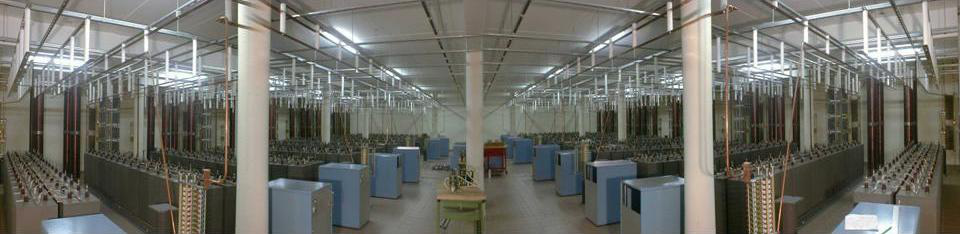
\includegraphics[scale=0.3]{Figures/cmi/powersupply_pulsed.png}
   \end{figure}

   Installation champs continus  GRENOBLE: 24 MW,  35  Tesla
   \vskip-0.3cm

 \begin{columns}[c]
  \begin{column}{8cm}
   \begin{figure}[H]
    \centering
    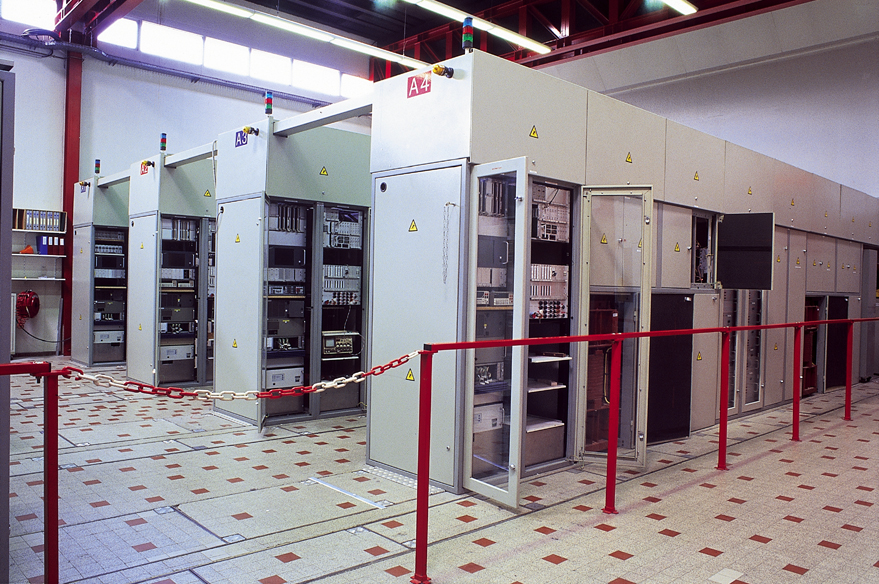
\includegraphics[scale=0.2]{Figures/cmi/powersupply.png}
   \end{figure}
  \end{column}

  \begin{column}{5cm}
   \begin{figure}[H]
    \centering
    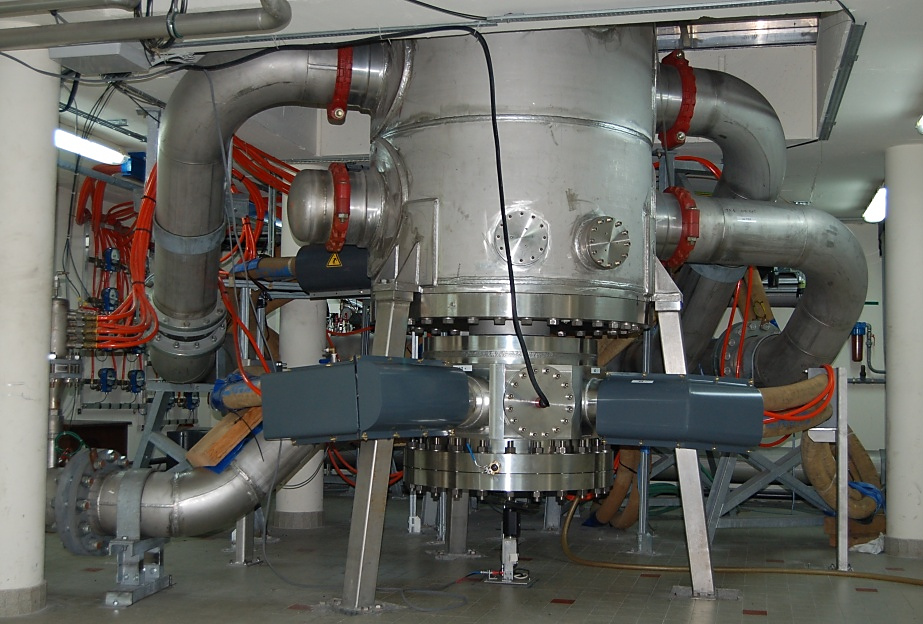
\includegraphics[scale=0.4]{Figures/cmi/magnet.png}
   \end{figure}
  \end{column}
 \end{columns}

\end{frame}

\begin{frame}{Champs Magn\'etiques Intenses}
%dire que c'est comme NHFML in Florida
\begin{columns}[c]
 \begin{column}{5.9cm}
  \begin{alertblock}{ \begin{small} Grand équipement francais \end{small}}
    \begin{small}
   \begin{itemize}
    \item Champs magnétiques intenses : à partir de 24 T .
    \item À Grenoble le champs magnétiques d'intensité maximum : 35 T
      (objectif 40-45T).
   \end{itemize}
    \end{small}
  \end{alertblock}
 \end{column}
 \begin{column}{5.9cm}
  \begin{block}{ \begin{small} Domaine d'application \end{small}}
   \begin{small}
   \begin{itemize}
    \item Science du magnétisme ;
    \item Physique du solide  (Résonance Magnétique Nucléaire) ;
    \item Supraconductivité appliquée.
   \end{itemize}
    \end{small}
  \end{block}
 \end{column}
\end{columns}

\begin{columns}[c]
 \begin{column}{2.5cm}
  \begin{figure}[H]
   \centering
   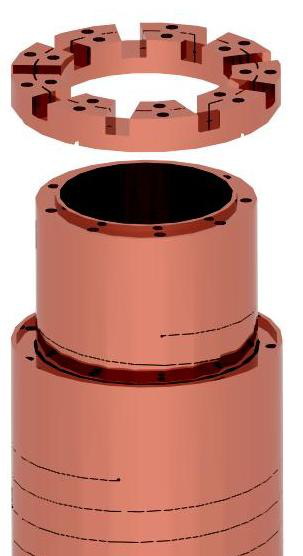
\includegraphics[scale=0.2]{Figures/cmi/Helices.png}
    \caption{Helix}
  \end{figure}
 \end{column}
 \begin{column}{3.4cm}
   \begin{figure}[H]
   \centering
   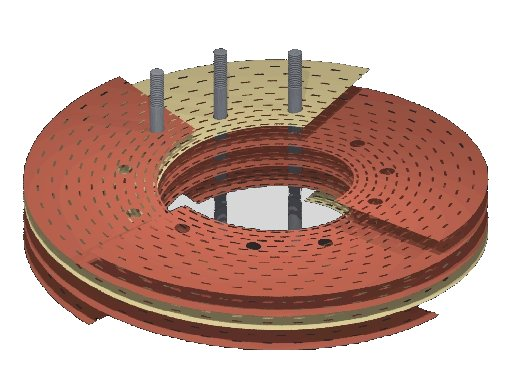
\includegraphics[scale=0.2]{Figures/cmi/Bitter.png}
    \caption{Bitter}
  \end{figure}
 \end{column}
 \begin{column}{4.6cm}
  \begin{block}{\begin{small} Champs magnétique \end{small}}
   \begin{small}
   \begin{itemize}
    \item Champs terrestre : $5.8 \cdot 10^{-4} T$ .
    \item Supraconducteurs : $24 T$ .
    \item \textcolor{red!80}{Champs continus : $35 T$  .}
    \item Champs pulsés : $90 T$ .
   \end{itemize}
  \end{small}
  \end{block}

 \end{column}
\end{columns}

\end{frame}

%\subsection{Magnet study requires multi-physics modeling}
\begin{frame}{Champs Magnétiques Intenses}
  \vspace*{-0.5cm}
  \begin{columns}[c]
    \begin{column}{.5\linewidth}

      \begin{block}{Simulation des électro-aimants}
        % dire a la fin avant la limitation des modeles qu'on va s'interesser a electro-heat
        \begin{itemize}
        \item Champs magnétique intense
          \begin{itemize}
          \item Densité de courant $j=-\sigma \nabla V$
          \item Électrostatique/Magnétostatique
          \end{itemize}

        \item Éffet Joule
          \begin{itemize}
          \item Dissipation de l'énergie thermique
          \item $\rightarrow$ \textcolor{red}{Température} \\
          \end{itemize}

        \item Refroidissement des électro-aimants
          \begin{itemize}
          \item Échanges thermiques entre le conducteur et l'eau
          \item $\rightarrow$ \textcolor{red}{thermo-hydraulique } \\
          \end{itemize}

        \item Stress mécanique
          \begin{itemize}
            % \item Laplace force (induced by magnetic field)
          \item Forces de Lorentz, Dilatation thermique
          \item $\rightarrow$ \textcolor{red}{Mécanique - Elasticité} \\
          \end{itemize}
        \end{itemize}
      \end{block}

    \end{column}
    \begin{column}{5cm}
      \vspace*{-0.3cm}
      \begin{figure}[H]
        \centering
        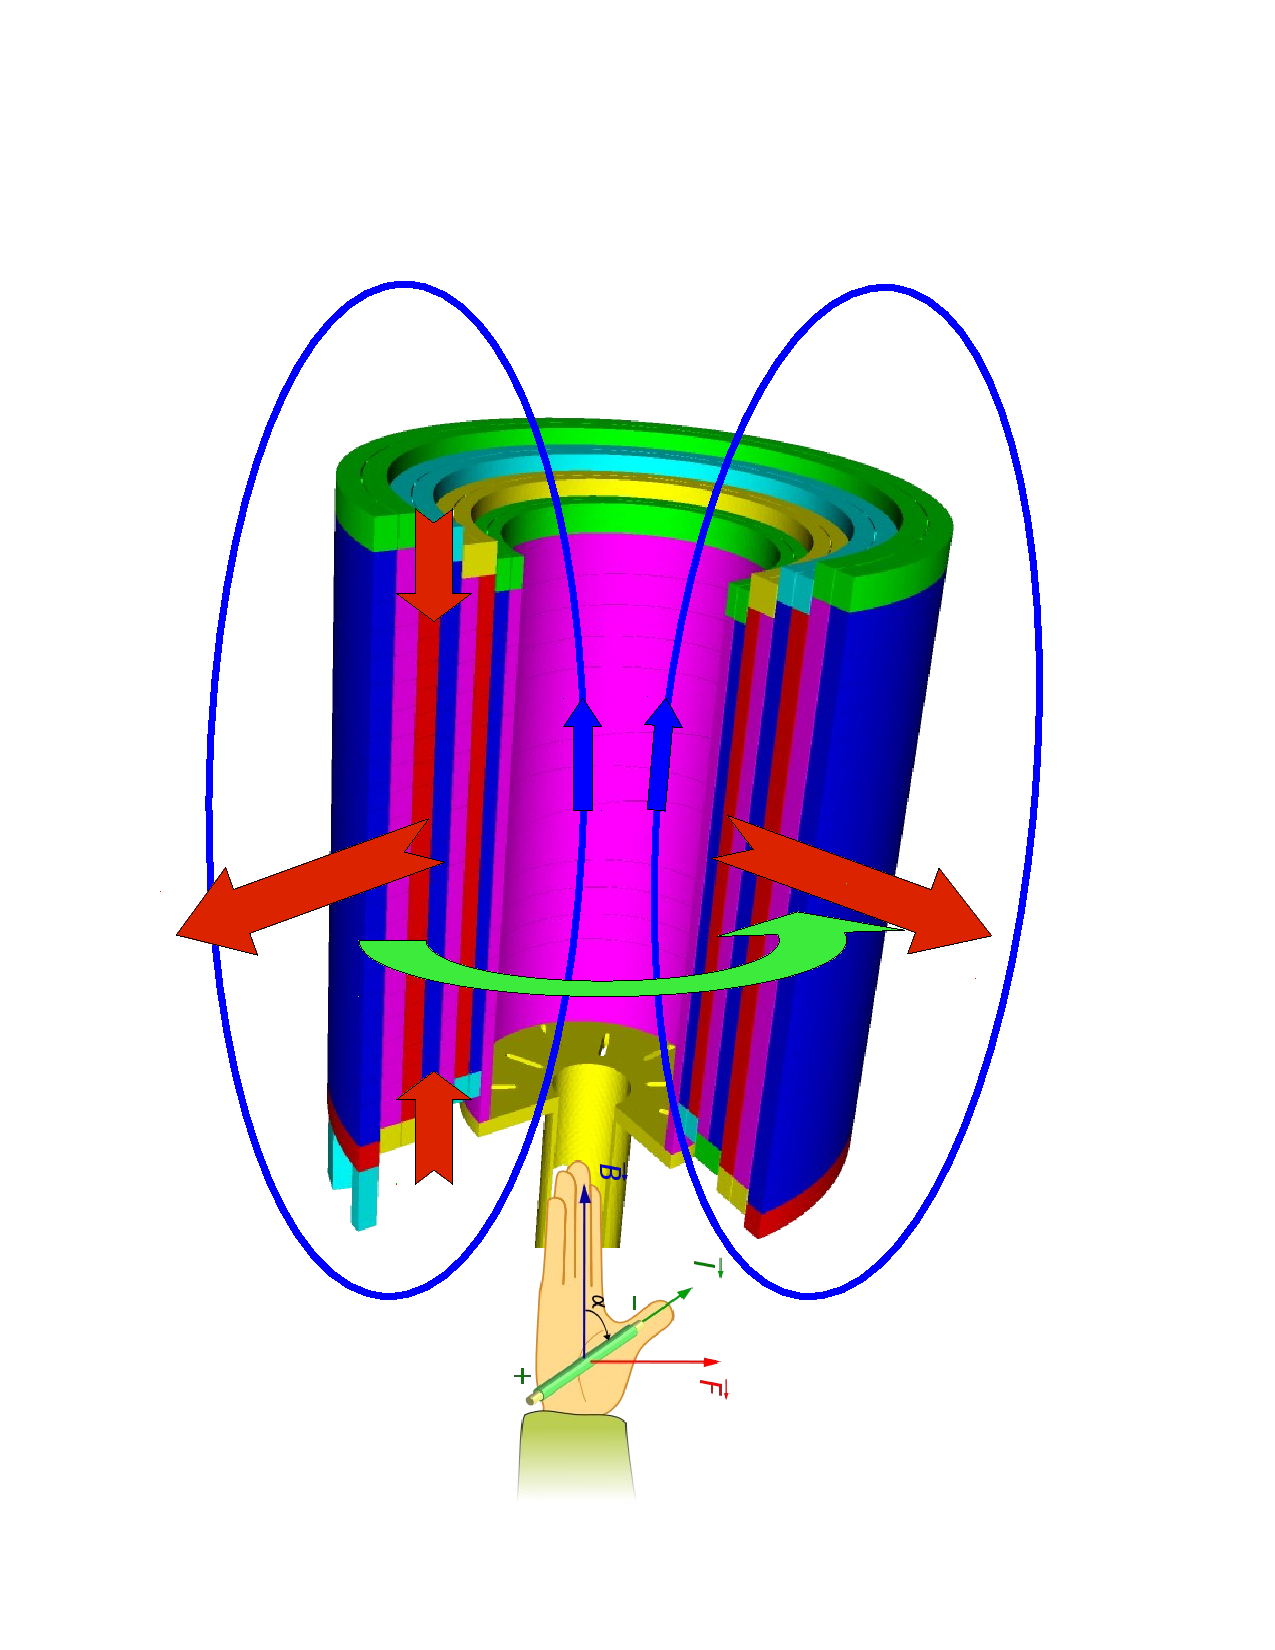
\includegraphics[scale=0.28]{Figures/cmi/Schema_Forces.pdf}
      \end{figure}
      % \begin{alertblock}{Need numerical simulation}
      % \item design models achieved their limits
      % \end{alertblock}
    \end{column}
  \end{columns}
\end{frame}

\begin{frame}{Champs Magnétiques Intenses}
  \begin{block}{Objectifs}
    \begin{columns}[c]
      \column{.5\linewidth}

      \begin{itemize}
      \item Hiérarchie de modèles
      \item Réduction de modèles (simulation temps réel fiable)
      \item Optimisation du design des électro-aimants
      \end{itemize}


      \column{.5\linewidth}
      \begin{itemize}
      \item Contrôle  des électro-aimants
      \item Quantification d'incertitudes :
        \begin{itemize}
        \item Analyse de sensibilité
        \item Estimation de quantile
        \end{itemize}
      \item Optimisation sous incertitudes
      \end{itemize}
  \end{columns}
    \end{block}
    \begin{columns}[c]
      \column{.3\linewidth}
      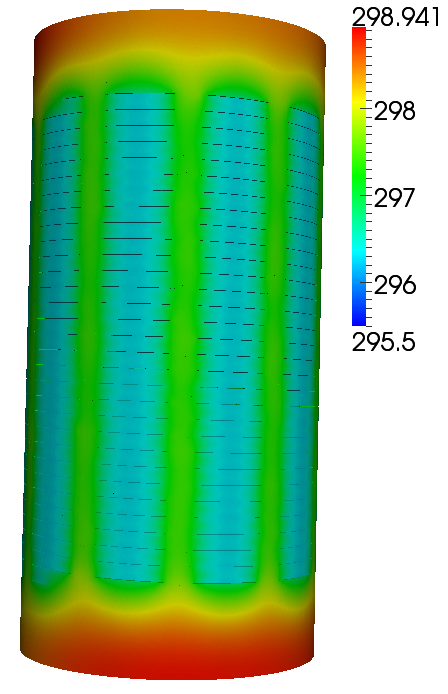
\includegraphics[height=.5\textheight]{Figures/cmi/temperature_HR_Bosse_1.png}
      \column{.3\linewidth}
      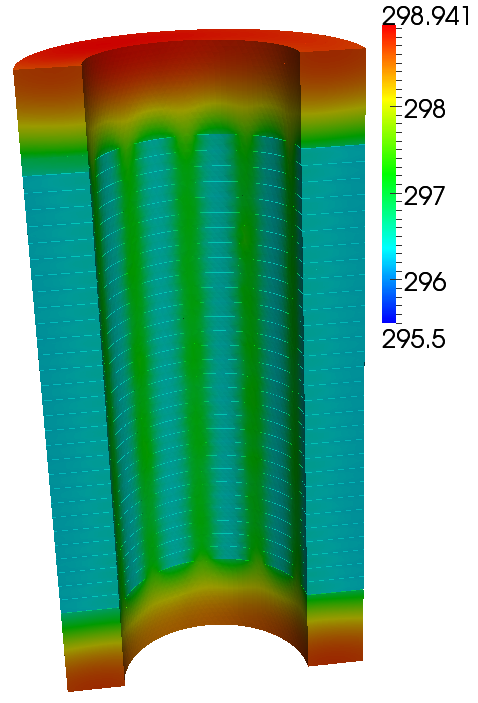
\includegraphics[height=.5\textheight]{Figures/cmi/temperature_HR_Bosse_cut1.png}
      \column{.3\linewidth}
      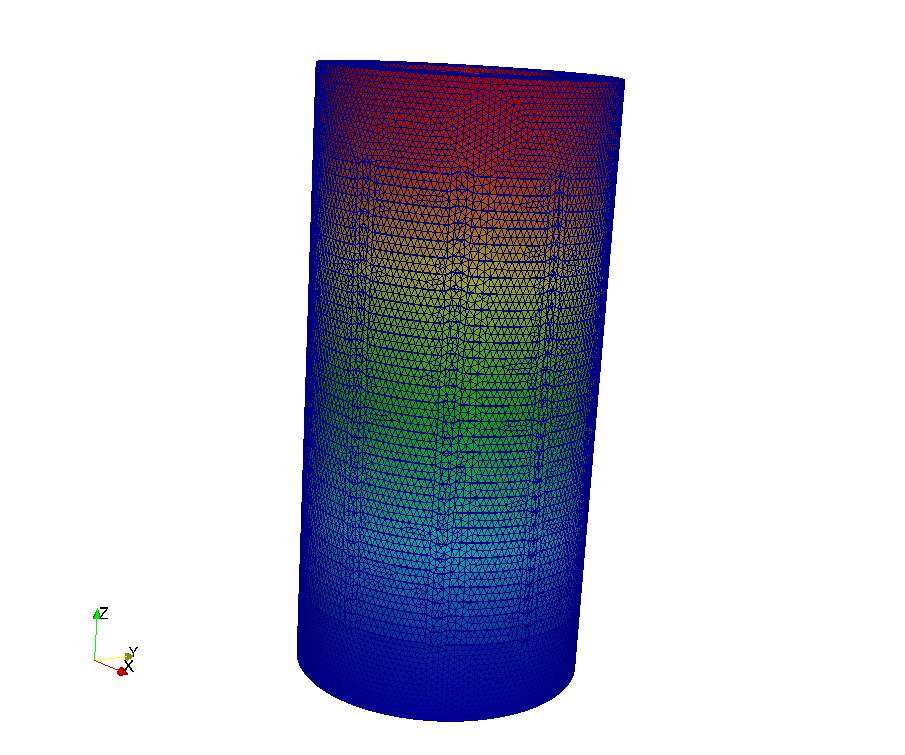
\includegraphics[height=.5\textheight]{Figures/cmi/potentiel_HR_Bosse_mesh1.png}
    \end{columns}

\end{frame}

%%% Local Variables: 
%%% mode: latex
%%% TeX-master: "slides-math-formations-metiers"
%%% End: 
